\chapter{स्तनधारियों का लैंगिक जनन}\label{ch:b2:mammal-reproduction}

मानव अंडाणु मिलिमीटर के दसवें भाग जितना चौड़ा है, यानी शरीर की सबसे बड़ी
कोशिका; और शुक्राणु एक चालक-पूँछ वाला केंद्रक है, उन तीस करोड़ में से
एक जो एक साथ छोड़े जाते हैं, जिनमें से कुछ दर्जन अंडाणु तक पहुँचेंगे और
एक उसमें घुसेगा। सप्ताह भर में वह निषेचित अंडाणु ऐसी खोखली गेंद बन जाता
है जो गर्भाशय की भित्ति में धँस जाती है और अपनी ही बाहरी कोशिकाओं से एक
अंग --- \omterm{def:b2:mammal-reproduction:placenta}{अपरा} --- गढ़ लेती है, जिससे उसकी माता उसे नौ महीने
खिलाएगी। फिर वह जन्म लेता है और दूध पर पलता है। हर स्तनधारी यह करता है;
और कोई दूसरा प्राणी यह सब नहीं करता। यह अध्याय युग्मकों से निषेचन तक,
भ्रूण से \omterm{def:b2:mammal-reproduction:implantation}{रोपण} तक, और उस जीव को गर्भावधि, जन्म तथा
स्तनपायन के आरपार ले चलता है, और अंत में बताता है कि दोनों लिंग कैसे बनते हैं।

\section{जनद और युग्मक}

\begin{definition}[वृषण और शुक्राणुजनन]\label{def:b2:mammal-reproduction:testis}
\index{शुक्राणुजनन}\index{शुक्रजनक नलिका}\index{सर्टोली कोशिका}\index{लाइडिग कोशिका}
\emph{वृषण} \emph{शुक्रजनक नलिकाओं} का पिंड है, जो कुल मिलाकर कई
सौ मीटर लंबी हैं और जिनकी भित्तियाँ शुक्राणु बनाती हैं; और नलिकाओं के बीच
\emph{लाइडिग कोशिकाएँ} पड़ी हैं, जो टेस्टोस्टेरोन बनाती हैं। नलिका की
भित्ति में बाहरी किनारे की \emph{शुक्राणुजन} कोशिकाएँ समसूत्री विभाजन से
विभाजित होती हैं, एक स्तंभ-आबादी बनाए रखती हैं और कोशिकाएँ भीतर की ओर
भेजती हैं; ये बढ़कर प्राथमिक \emph{शुक्राणुकोशिकाएँ} बनती हैं, जो
\omterm{def:b2:meiosis-heredity:meiosis}{अर्धसूत्री विभाजन} I (दो द्वितीयक शुक्राणुकोशिकाओं तक) और
\omterm{def:b2:meiosis-heredity:meiosis}{अर्धसूत्री विभाजन} II (चार \omterm{def:b2:meiosis-heredity:meiosis}{अगुणित} \emph{शुक्राणुप्रसू} तक) से गुज़रती हैं;
और शुक्राणुप्रसू अपना अधिकांश कोशिकाद्रव्य त्याग देते हैं, अपना केंद्रक
संघनित करते हैं, एक कशाभ उगाते हैं और केंद्रक पर \emph{एक्रोसोम} की टोपी
चढ़ा लेते हैं, यानी एंजाइमों की एक पुटिका, और यों \emph{शुक्राणु} बनकर
गुहा में छोड़ दिए जाते हैं। बड़ी \emph{सर्टोली कोशिकाएँ} पूरी भित्ति
लाँघती हैं, जनन कोशिकाओं की परिचर्या करती हैं और आपस की दृढ़ संधियों से
ऐसा \emph{रक्त--वृषण अवरोध} बनाती हैं जो प्रतिरक्षा तंत्र को उन
कोशिकाओं से दूर रखता है जो पहली बार यौवनारंभ पर प्रकट होती हैं। पूरे
क्रम में किसी पुरुष में लगभग \num{64} दिन लगते हैं और वह यौवनारंभ से
बुढ़ापे तक प्रतिदिन कोई $10^{8}$ शुक्राणु देता है। शुक्राणु वृषण से
अचल निकलते हैं और \emph{अधिवृषण} में दो सप्ताह तक परिपक्व होते हैं।
\end{definition}

\begin{omfigure}
\begin{tikzpicture}[every node/.style={font=\scriptsize}]
  % tubule cross-section: concentric layers
  \draw[thick, fill=omExo!15] (0,0) circle (2.5);
  \draw[thick, fill=omExo!8] (0,0) circle (2.2);
  \draw[thick, fill=omDef!10] (0,0) circle (1.6);
  \draw[thick, fill=omProp!12] (0,0) circle (1.0);
  \draw[thick, fill=white] (0,0) circle (0.45);
  % cells
  \foreach \a in {0,30,...,330} \draw[thick, fill=omDef!40] (\a:2.0) circle (0.13);
  \foreach \a in {15,45,...,345} \draw[thick, fill=omDef!70] (\a:1.32) circle (0.16);
  \foreach \a in {0,20,...,340} \draw[thick, fill=omProp!60] (\a:0.75) circle (0.08);
  \foreach \a in {10,40,...,340} \draw[thick, omProp!80!black] (\a:0.45) -- (\a:0.15);
  % Sertoli cell: tall wedge
  \draw[thick, omExo!70!black, fill=omExo!40, opacity=0.6] (100:2.2) .. controls (90:1.6) and (95:0.9) .. (92:0.5) .. controls (80:0.9) and (75:1.6) .. (72:2.2) -- cycle;
  % Leydig cells outside
  \foreach \p in {(2.9,0.8),(3.1,0.3),(2.8,-0.3)} \draw[thick, fill=omThm!40] \p circle (0.14);
  % labels
  \draw (2.0,0) -- (3.6,-0.5) node[right, align=left] {बाहरी किनारे पर\\शुक्राणुजन ($2n$)};
  \draw (1.32,-0.7) -- (3.6,-1.5) node[right, align=left] {प्राथमिक शुक्राणुकोशिकाएँ\\(अर्धसूत्री विभाजन I)};
  \draw (0.75,-0.4) -- (3.6,-2.4) node[right, align=left] {शुक्राणुप्रसू ($n$)};
  \draw (0.3,-0.2) -- (3.6,-3.1) node[right, align=left] {गुहा में शुक्राणु};
  \draw (2.95,0.55) -- (3.6,0.6) node[right, align=left] {लाइडिग कोशिकाएँ:\\टेस्टोस्टेरोन};
  \draw (88:1.4) -- (3.6,1.8) node[right, align=left] {भित्ति लाँघती सर्टोली कोशिका};
  \node[anchor=east, align=right] at (-2.7,0) {बाहर\\(आधार पटलिका)};
\end{tikzpicture}

{\small किसी \omterm{def:b2:mammal-reproduction:testis}{शुक्रजनक नलिका} की अनुप्रस्थ काट। जनन कोशिकाएँ बाहरी
भित्ति से (शुक्राणुजन) भीतर की ओर (शुक्राणुकोशिकाएँ,
शुक्राणुप्रसू, गुहा में शुक्राणु) परिपक्व होती हैं, और \omterm{def:b2:mammal-reproduction:testis}{सर्टोली कोशिकाएँ}
उन्हें सहारा देती हैं; नलिकाओं के बीच की \omterm{def:b2:mammal-reproduction:testis}{लाइडिग कोशिकाएँ} टेस्टोस्टेरोन बनाती हैं।}
\end{omfigure}

\begin{omfigure}
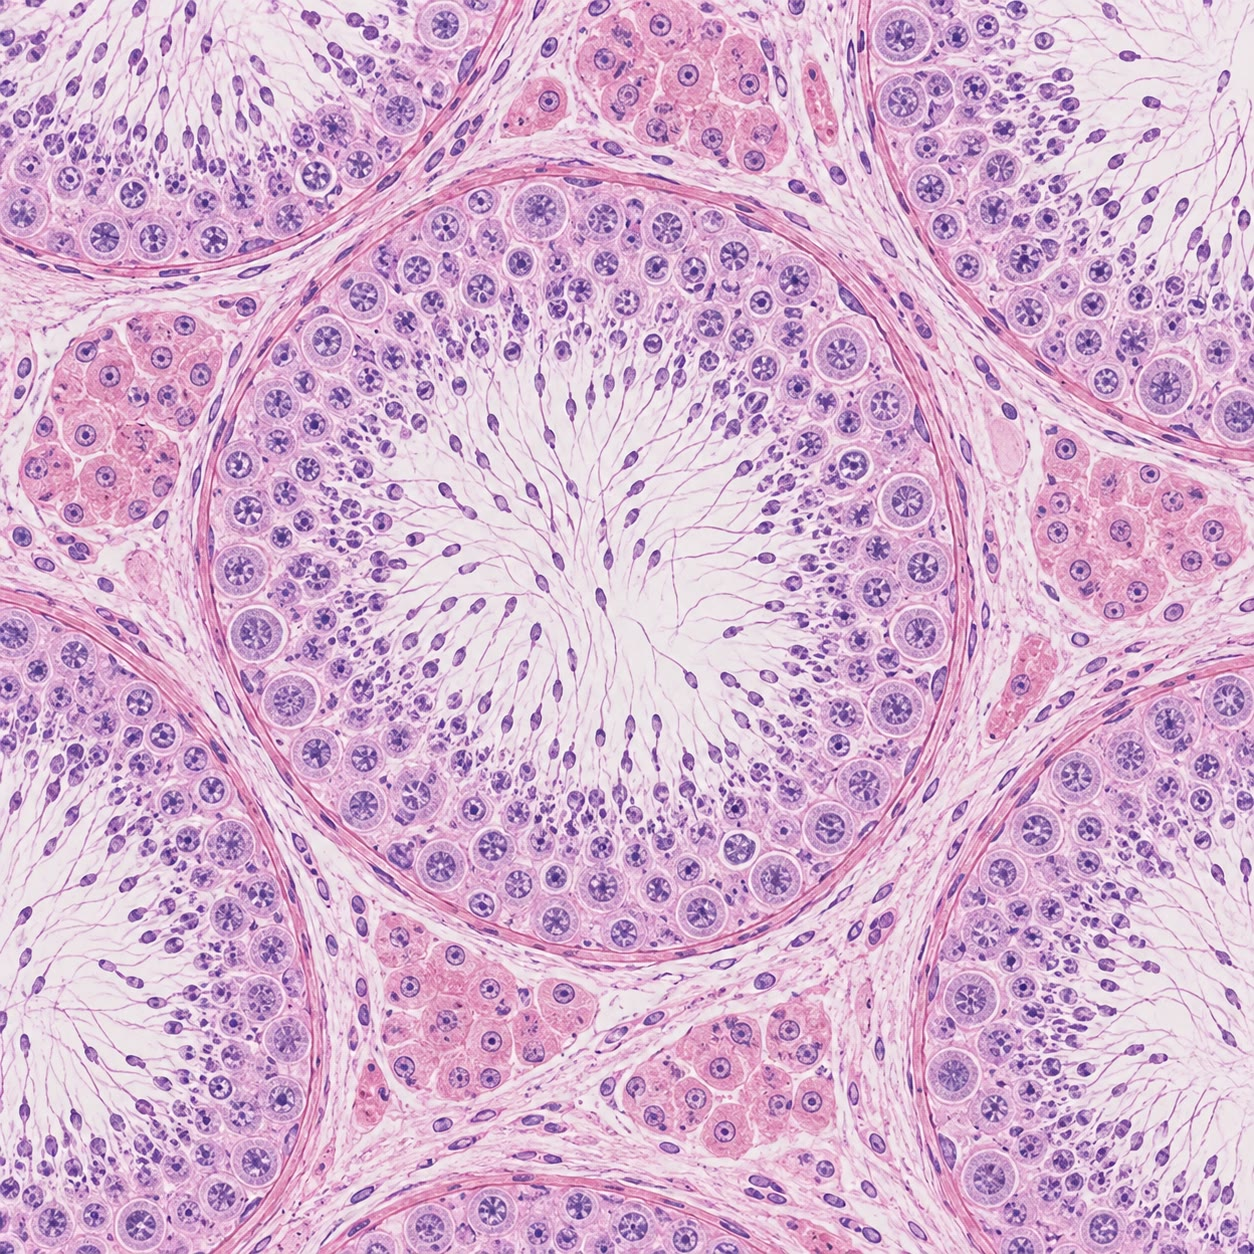
\includegraphics[width=0.42\linewidth]{images/book4/ai/b4-08-testis-histology.jpg}\hspace{0.04\linewidth}
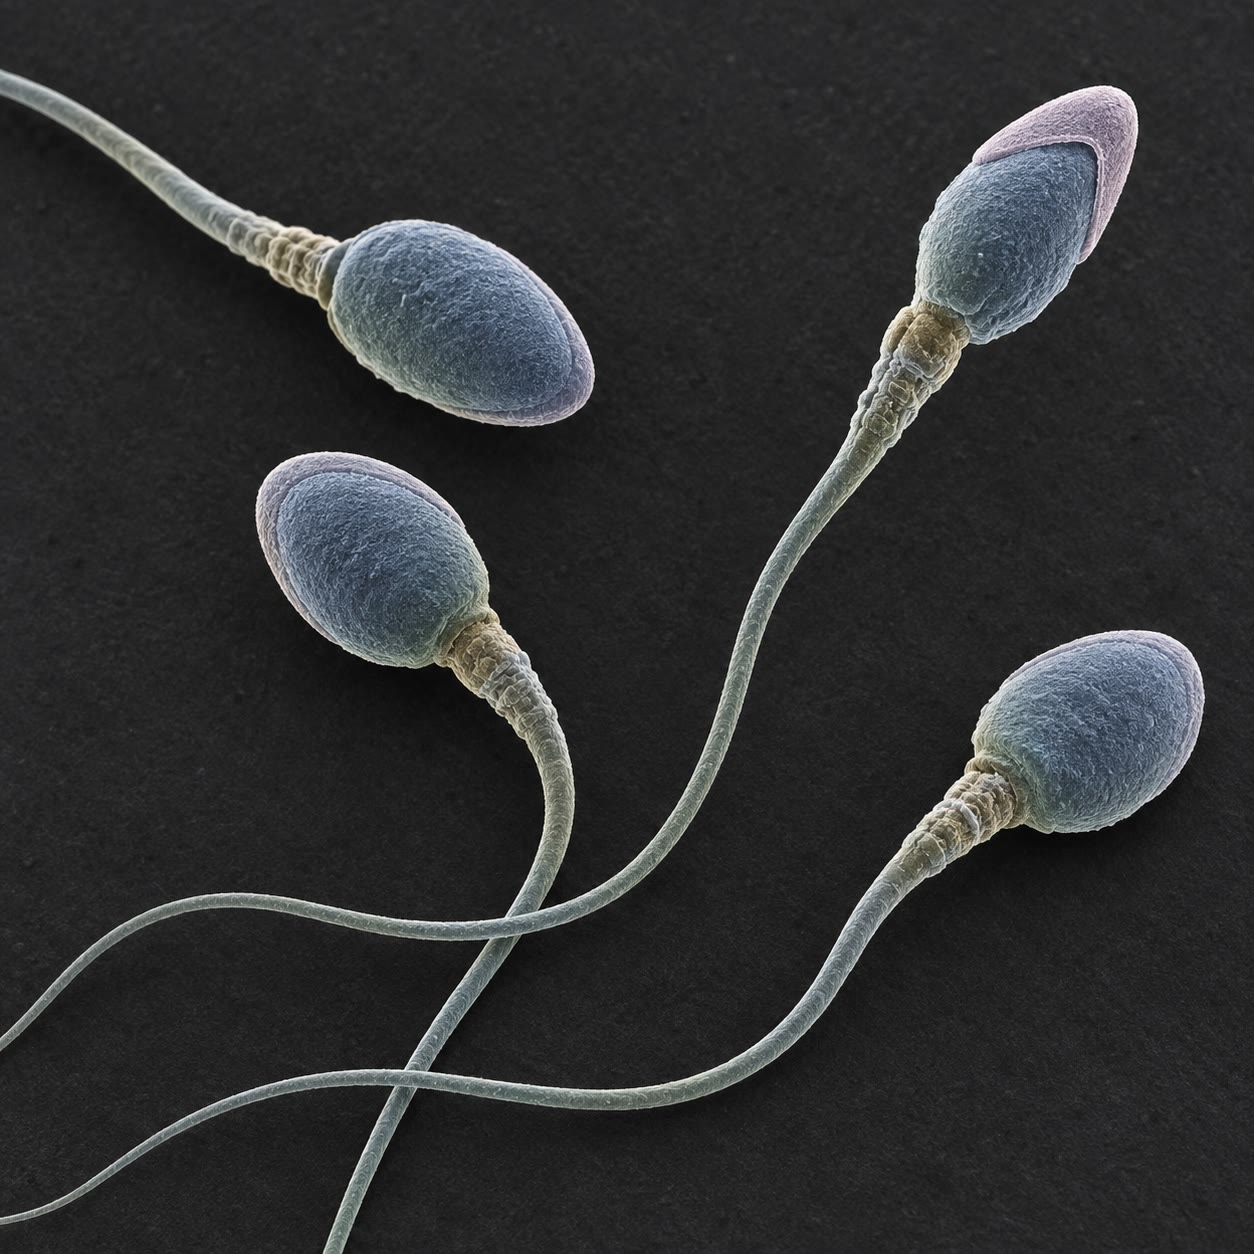
\includegraphics[width=0.42\linewidth]{images/book4/ai/b4-08-sperm-sem.jpg}

{\small बाएँ: काट में \omterm{def:b2:mammal-reproduction:testis}{शुक्रजनक नलिकाएँ}, जिनमें जनन कोशिकाएँ
भित्ति से गुहा तक परतों में हैं। दाएँ: क्रमवीक्षी इलेक्ट्रॉन
सूक्ष्मदर्शी के नीचे शुक्राणु, जिनके शीर्षों पर एक्रोसोम की टोपी दिख रही
है।}
\end{omfigure}

\begin{definition}[अंडाशय और अंडाणुजनन]\label{def:b2:mammal-reproduction:ovary}
\index{अंडाणुजनन}\index{पुटक}\index{अंडोत्सर्ग}\index{पीत पिंड}
अंडाणुजनन लगभग हर बात में \omterm{def:b2:mammal-reproduction:testis}{शुक्राणुजनन} का दर्पण-प्रतिबिंब
है। \emph{अंडाणुजन} केवल भ्रूण में गुणित होते हैं: जन्म तक कोई बालिका
लगभग दस लाख प्राथमिक \emph{अंडाणुकों} का भंडार ढोती है, और हर एक
\omterm{def:b2:meiosis-heredity:meiosis}{अर्धसूत्री विभाजन} की \omterm{prop:b2:meiosis-heredity:stages}{पूर्वावस्था I} में ठहरा और कोशिकाओं की एक ही परत में
लिपटा है --- यानी कोई \emph{आद्य पुटक} --- और नए कभी नहीं
बनते। यौवनारंभ से हर महीने पुटकों का एक दल बढ़ता है:
अंडाणुक बड़ा होता है, चारों ओर की \emph{कणिकामय} कोशिकाएँ गुणित होकर
परतें बनाती हैं, एक बाहरी \emph{थीका} बनता है, द्रव भरी एक गुहा
खुलती है (यानी \emph{ग्राफ़ी पुटक}, दो सेंटीमीटर चौड़ा), और
प्रायः कोई एक ही \emph{अंडोत्सर्ग} तक पहुँचता है: वह अंडाणुक, जो अब जाकर
\omterm{def:b2:meiosis-heredity:meiosis}{अर्धसूत्री विभाजन} I पूरा करता है और मध्यावस्था II में फिर ठहर जाता है,
अपनी कणिकामय कोशिकाओं के प्रभामंडल सहित अंडवाहिनी में निकाल दिया जाता
है। ख़ाली हुआ पुटक \emph{पीत पिंड} बन जाता है, यानी
प्रोजेस्टेरोन की एक अस्थायी ग्रंथि। \omterm{def:b2:meiosis-heredity:meiosis}{अर्धसूत्री विभाजन} एक अंडाणु और तीन
नन्हे ध्रुवीय पिंड बनाता है --- सारा कोशिकाद्रव्य एक ही कोशिका को जाता
है --- और \omterm{def:b2:meiosis-heredity:meiosis}{अर्धसूत्री विभाजन} II तभी पूरा होता है जब कोई शुक्राणु
घुसे। उन दस लाख अंडाणुकों में से जीवन भर में लगभग \num{400} अंडोत्सर्जित
होते हैं; बाक़ी क्षीण हो जाते हैं
(\emph{पुटकनाश}), और जब वह भंडार चुक जाता है, कोई पचास की आयु में, तब
चक्र रुक जाते हैं: यही रजोनिवृत्ति है।
\end{definition}

\begin{omfigure}
\begin{tikzpicture}[every node/.style={font=\scriptsize}, >=stealth]
  % timeline of oogenesis vs spermatogenesis
  \draw[thick, ->] (0,3.0) -- (12.6,3.0); \node[anchor=west] at (12.6,3.0) {आयु};
  \foreach \x/\l in {0/{भ्रूण}, 2.2/{जन्म}, 4.6/{यौवनारंभ}, 10.2/{$\sim$50 वर्ष}}
    \draw (\x,3.1) -- (\x,2.9) node[above=0.15cm] {\l};
  % oogenesis line
  \node[anchor=east, omThm] at (-0.2,1.5) {अंडाणुजनन};
  \draw[very thick, omThm] (0,1.5) -- (1.6,1.5); \node[above, omThm, align=center] at (0.8,1.55) {अंडाणुजन\\गुणित होते हैं};
  \draw[very thick, omThm, dashed] (1.6,1.5) -- (4.6,1.5); \node[below, omThm] at (3.1,1.45) {पूर्वावस्था I में ठहराव};
  \draw[very thick, omThm] (4.6,1.5) -- (10.2,1.5); \node[above, omThm, align=center] at (7.4,1.55) {महीने में एक अंडोत्सर्ग;\\अर्धसूत्री विभाजन I अंडोत्सर्ग पर पूरा, II निषेचन पर};
  \fill[omThm] (10.2,1.5) circle (0.07); \node[below, omThm] at (10.2,1.45) {भंडार चुक गया};
  % spermatogenesis line
  \node[anchor=east, omDef] at (-0.2,0.3) {शुक्राणुजनन};
  \draw[very thick, omDef, dashed] (0,0.3) -- (4.6,0.3); \node[above, omDef] at (2.3,0.35) {शुक्राणुजन निष्क्रिय};
  \draw[very thick, omDef, ->] (4.6,0.3) -- (12.6,0.3); \node[above, omDef] at (8.6,0.35) {सतत: प्रतिदिन $10^{8}$ शुक्राणु, हर एक 64 दिन, स्तंभ कोशिकाओं से};
\end{tikzpicture}

{\small काल में दोनों युग्मकजनन। अंडाणुक सब जन्म से पहले बन जाते हैं और
किसी परिमित भंडार से एक-एक करके छोड़े जाते हैं; जबकि शुक्राणु पूरे वयस्क
जीवन भर स्तंभ कोशिकाओं से लगातार बनते रहते हैं।}
\end{omfigure}

\begin{omfigure}
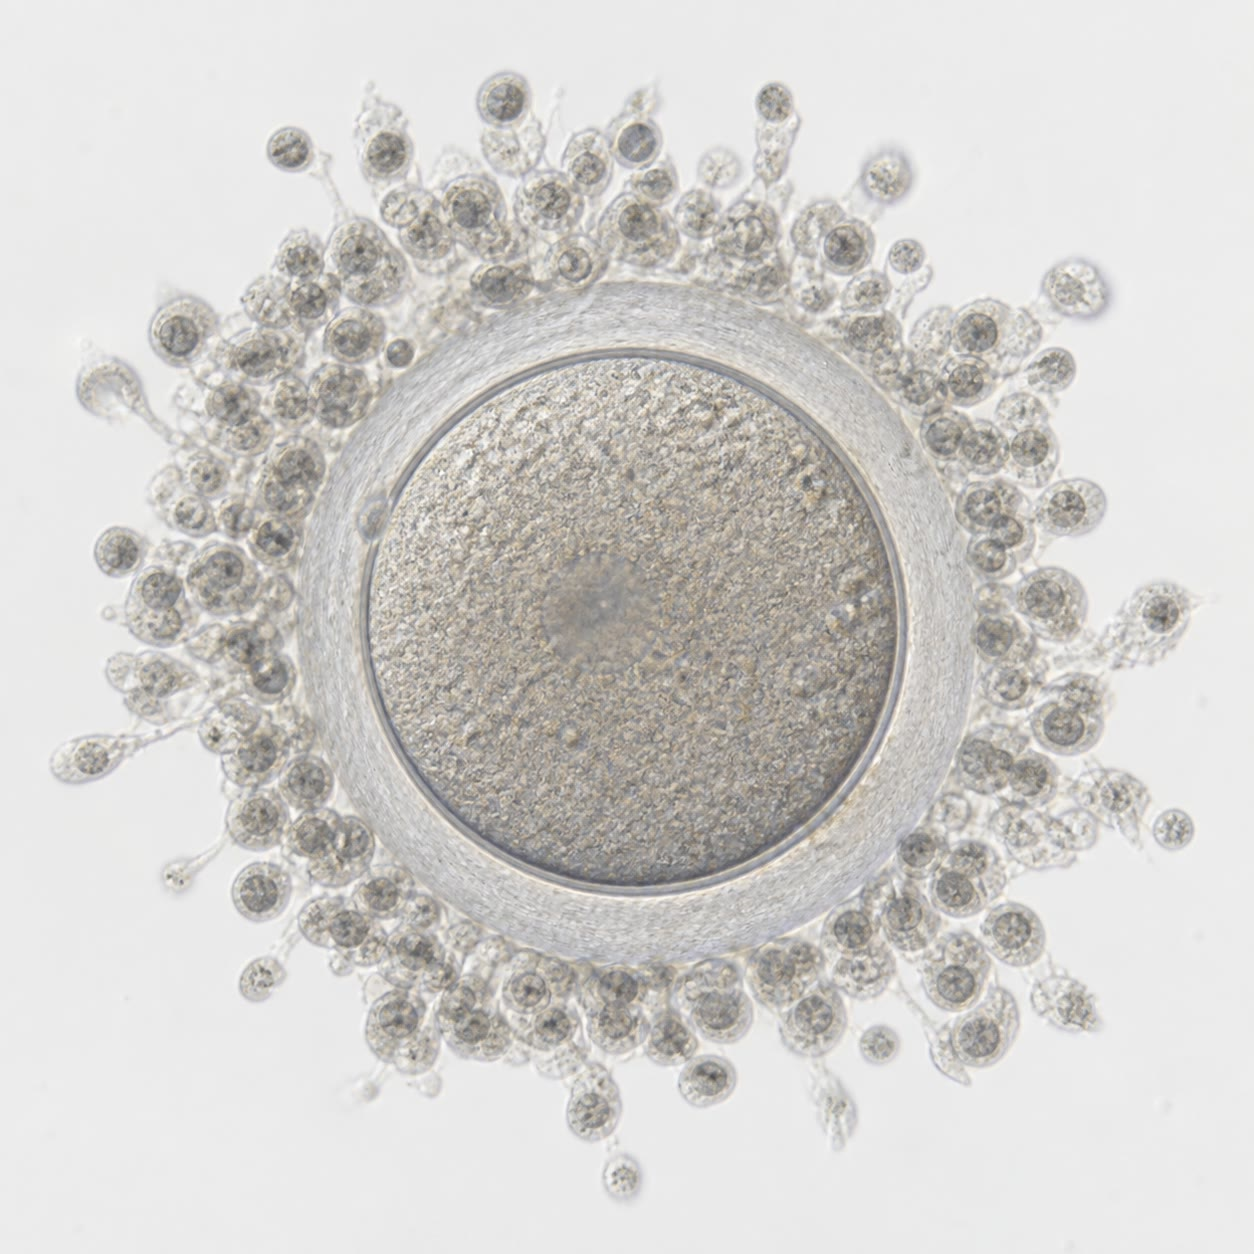
\includegraphics[width=0.46\linewidth]{images/book4/ai/b4-08-oocyte.jpg}

{\small कोई अंडोत्सर्जित अंडाणुक: वह कोशिका, उसका पारदर्शी आवरण
(\omterm{prop:b2:mammal-reproduction:fertilisation}{पारदर्शी पटल}), और कणिकामय कोशिकाओं का वह बादल जो उसके साथ
\omterm{def:b2:mammal-reproduction:ovary}{पुटक} से निकला।}
\end{omfigure}

\section{निषेचन}

\begin{proposition}[निषेचन के चरण]\label{prop:b2:mammal-reproduction:fertilisation}
\index{निषेचन!स्तनधारियों में}\index{एक्रोसोम अभिक्रिया}\index{पारदर्शी पटल}\index{वल्कुटीय अभिक्रिया}
योनि में छोड़े गए शुक्राणु --- कोई $3\times 10^{8}$ --- ग्रीवा का
श्लेष्म पार करते हैं, गर्भाशय के संकुचनों से ऊपर बुहार दिए जाते हैं, और
कुछ सौ घंटे भर में अंडवाहिनी की तुंबिका तक पहुँच जाते हैं, जहाँ
अंडाणु एक दिन प्रतीक्षा करता है। रास्ते में शुक्राणु
\emph{सक्षमन} से गुज़रते हैं: मादा मार्ग के स्राव उनकी
झिल्लियों से आवरण-प्रोटीन उतार देते हैं और उन्हें अतिसक्रिय बना देते
हैं। अंडाणु पर कोई शुक्राणु कणिकामय कोशिकाओं से होकर ठेलता है,
\emph{\omterm{prop:b2:mammal-reproduction:fertilisation}{पारदर्शी पटल}} के किसी ग्लाइकोप्रोटीन से बँधता है, और
\emph{\omterm{prop:b2:mammal-reproduction:fertilisation}{एक्रोसोम अभिक्रिया}} से गुज़रता है, यानी ऐसे एंजाइम छोड़ता है जो
उस पटल से होकर एक रास्ता पचा देते हैं; उसकी झिल्ली अंडाणु की झिल्ली से
संलयित होती है और शुक्राणु-केंद्रक भीतर चला जाता है।
अंडाणु सेकंडों में उत्तर देता है: कैल्सियम उसमें से बह जाता है, और
वल्कुटीय कणिकाएँ ऐसे एंजाइम छोड़ती हैं जो उस पटल को कड़ा कर देते हैं और
उसके शुक्राणु-ग्राही उतार देते हैं --- यही \emph{\omterm{prop:b2:mammal-reproduction:fertilisation}{वल्कुटीय अभिक्रिया}} है,
यानी बहुशुक्राणुता का अवरोध। अंडाणु \omterm{def:b2:meiosis-heredity:meiosis}{अर्धसूत्री विभाजन} II पूरा करता है,
दूसरा ध्रुवीय पिंड त्यागता है, और दोनों \omterm{def:b2:meiosis-heredity:meiosis}{अगुणित} \emph{पूर्वकेंद्रक} अपना
DNA प्रतिकृत करते हैं, पास आते हैं और पहले समसूत्री विभाजन में घुसते
हैं: युग्मनज एक दिन का हो चुका है। जाति-विशिष्टता उस पटल के प्रोटीनों में
है, और इसीलिए किसी चूहे का शुक्राणु किसी मानव अंडाणु में नहीं घुसता।
\end{proposition}
\begin{proof}[प्रमाण-सामग्री]
एडवर्ड्स और स्टेप्टो (1978) ने \omterm{def:b2:mammal-reproduction:ovary}{अंडोत्सर्ग} से कुछ ही पहले अंडाशय से
निकाले गए किसी मानव अंडाणुक को सक्षमित शुक्राणुओं से किसी तश्तरी में
निषेचित किया, उस भ्रूण को आठ कोशिकाओं तक संवर्धित किया और
गर्भाशय में लौटा दिया, जहाँ वह रोपित हुआ और जन्मा: यही पात्रे निषेचन है।
ऊपर के क्रम का हर चरण पहले समुद्री अर्चिन और चूहे में सुलझाया गया था,
जहाँ संलयन, कैल्सियम तरंग और वल्कुटीय कणिकाओं का मोचन देखा जा सकता है;
और चूहे में \omterm{def:b2:genome-diversification:mutation}{उत्परिवर्तन} से पटल का एक ग्लाइकोप्रोटीन (ZP2 या ZP3) हटा
देने पर ऐसे अंडाणु बचते हैं जिनसे शुक्राणु बँध ही नहीं सकते।
\end{proof}

\begin{theorem}[एक अंडाणु को लाखों शुक्राणु क्यों चाहिए]\label{thm:b2:mammal-reproduction:poisson}
\index{बहुशुक्राणुता}
यदि छोड़े गए $N$ शुक्राणुओं में से हर एक स्वतंत्र रूप से किसी छोटी
प्रायिकता $\pi$ से अंडाणु की सतह तक पहुँचे, तो पहुँचने वालों की संख्या
$m = N\pi$ माध्य की पॉइसों है और कम से कम एक के पहुँचने की प्रायिकता है
\[
P = 1 - e^{-m}.
\]
$N = 3\times 10^{8}$ और $\pi \approx 10^{-8}$ के साथ $m \approx 3$
और $P \approx 0.95$; और $N = 2\times 10^{7}$ (यानी कम शुक्राणु-संख्या
की नैदानिक देहली) के साथ $m = 0.2$ और $P = 0.18$। वही
अंकगणित दिखाता है कि बहुशुक्राणुता का अवरोध क्यों अपरिहार्य है: जब
$P$ ऊँचा हो, तब कई शुक्राणु एक-दूसरे के सेकंडों के भीतर पहुँच जाते हैं,
और जिस अंडाणु में दो घुस जाएँ वह त्रिगुणित होकर मर जाएगा।
\end{theorem}
\begin{proof}
हर शुक्राणु $\pi$ सफलता-प्रायिकता का एक स्वतंत्र परीक्षण है;
सफलताओं की संख्या द्विपद है, जो बड़े $N$ और छोटे
$\pi$ के लिए $N\pi$ माध्य की पॉइसों है। शून्य सफलताओं की
प्रायिकता $e^{-m}$ है, इसलिए कम से कम एक की $1 - e^{-m}$; और
दो या अधिक की प्रायिकता $1 - e^{-m}(1 + m)$ है, यानी लगभग $0.8$ जब
$m = 3$ हो।
\end{proof}

\begin{omfigure}
\begin{tikzpicture}[every node/.style={font=\scriptsize}, >=stealth]
  \foreach \x/\lab in {0/{1. शुक्राणु पटल से\\बँधता है}, 3.3/{2. एक्रोसोम अभिक्रिया:\\एंजाइम रास्ता काटते हैं}, 6.6/{3. झिल्लियाँ संलयित;\\कैल्सियम तरंग}, 9.9/{4. वल्कुटीय अभिक्रिया:\\पटल कड़ा,\\अर्धसूत्री विभाजन II पूरा}} {
    \begin{scope}[xshift=\x cm]
      \draw[thick, fill=omThm!8] (0,0) circle (0.9);
      \draw[thick, omExo!70!black] (0,0) circle (1.15);
      \node[below, align=center] at (0,-1.3) {\lab};
    \end{scope}
  }
  % stage 1: sperm at zona
  \draw[thick, fill=omDef!50] (-1.45,0.1) ellipse (0.18 and 0.11); \draw[thick, omDef] (-1.63,0.1) .. controls (-2.0,0.4) and (-2.2,-0.2) .. (-2.5,0.1);
  % stage 2: sperm digging through zona
  \begin{scope}[xshift=3.3cm]
    \fill[white] (-1.2,0.0) circle (0.12);
    \draw[thick, fill=omDef!50] (-1.05,0.05) ellipse (0.18 and 0.11); \draw[thick, omDef] (-1.23,0.05) .. controls (-1.6,0.35) and (-1.8,-0.25) .. (-2.1,0.05);
    \foreach \a in {150,170,190,210} \draw[omProp, thick] (-1.2,0.0) -- ++(\a:0.25);
  \end{scope}
  % stage 3: fused, calcium wave
  \begin{scope}[xshift=6.6cm]
    \fill[white] (-1.15,0.0) circle (0.12);
    \draw[thick, fill=omDef!50] (-0.75,0.0) ellipse (0.18 and 0.11);
    \draw[thick, omDef] (-0.93,0.0) .. controls (-1.3,0.3) and (-1.5,-0.3) .. (-1.8,0.0);
    \foreach \r in {0.35,0.55,0.75} \draw[omProp, thick] (-0.75,0) ++(-60:\r) arc (-60:60:\r);
  \end{scope}
  % stage 4: hardened zona, polar body, pronuclei
  \begin{scope}[xshift=9.9cm]
    \draw[very thick, omExo!70!black] (0,0) circle (1.15);
    \draw[thick, fill=omDef!30] (-0.25,0.05) circle (0.2); \draw[thick, fill=omThm!30] (0.25,0.05) circle (0.2);
    \draw[thick, fill=omThm!20] (0.55,0.95) circle (0.12);
    \node[anchor=west] at (1.2,0.9) {ध्रुवीय पिंड};
    \draw (0.45,0.05) -- (1.2,-0.35); \node[anchor=west] at (1.2,-0.35) {दो पूर्वकेंद्रक};
  \end{scope}
\end{tikzpicture}

{\small चार चरणों में निषेचन: पटल से बँधना,
\omterm{prop:b2:mammal-reproduction:fertilisation}{एक्रोसोम अभिक्रिया}, संलयन तथा कैल्सियम तरंग, और वह \omterm{prop:b2:mammal-reproduction:fertilisation}{वल्कुटीय
अभिक्रिया} जो अंडाणु को बाक़ी शुक्राणुओं के लिए बंद कर देती है जबकि वह
अपना \omterm{def:b2:meiosis-heredity:meiosis}{अर्धसूत्री विभाजन} पूरा करता है।}
\end{omfigure}

\section{रोपण और अपरा}

\begin{definition}[विदलन, कोरकपुटी, रोपण]\label{def:b2:mammal-reproduction:implantation}
\index{कोरकपुटी}\index{पोषकोरक}\index{अंतःकोशिका पिंड}\index{रोपण}
युग्मनज हर बारह से बीस घंटे में बिना बढ़े विभाजित होता है
(\emph{विदलन}) जबकि वह अंडवाहिनी से नीचे ले जाया जाता है: दो कोशिकाएँ,
चार, आठ, सोलह की एक सघन गेंद (\emph{मोरुला}), और पाँचवें दिन तक लगभग सौ
कोशिकाओं की \emph{कोरकपुटी}: किसी गुहा के चारों ओर एक बाहरी परत, यानी
\emph{पोषकोरक}, और एक ओर कोशिकाओं का एक गुच्छा, यानी
\emph{अंतःकोशिका पिंड}। पोषकोरक \omterm{def:b2:mammal-reproduction:placenta}{अपरा} और झिल्लियाँ
गढ़ेगा; और अंतःकोशिका पिंड भ्रूण बनेगा
--- और इसी अवस्था पर निकाल लिया जाए तो भ्रूणीय स्तंभ कोशिकाएँ देता है।
छठे दिन वह कोरकपुटी अपने पटल से निकलती है, गर्भाशय के अस्तर से चिपकती
है, और पोषकोरक उस पर आक्रमण करता है: कोशिकाएँ संलयित होकर ऐसा
बहुकेंद्रकी मोर्चा बनाती हैं जो मातृ ऊतक पचाता है और मातृ
केशिकाएँ खोल देता है, इसलिए बारहवें दिन तक वह भ्रूण भित्ति में गड़ा और
मातृ रक्त में डूबा होता है। यही \emph{रोपण} है। वह केवल
प्रोजेस्टेरोन से तैयार किए गए गर्भाशय में, कुछ ही दिनों की एक खिड़की में,
सफल होता है; और सारे मानव गर्भाधानों में से लगभग आधे इस चरण पर या उससे
पहले विफल हो जाते हैं, प्रायः अंडाणु की गुणसूत्रीय त्रुटियों से।
\end{definition}

\begin{omfigure}
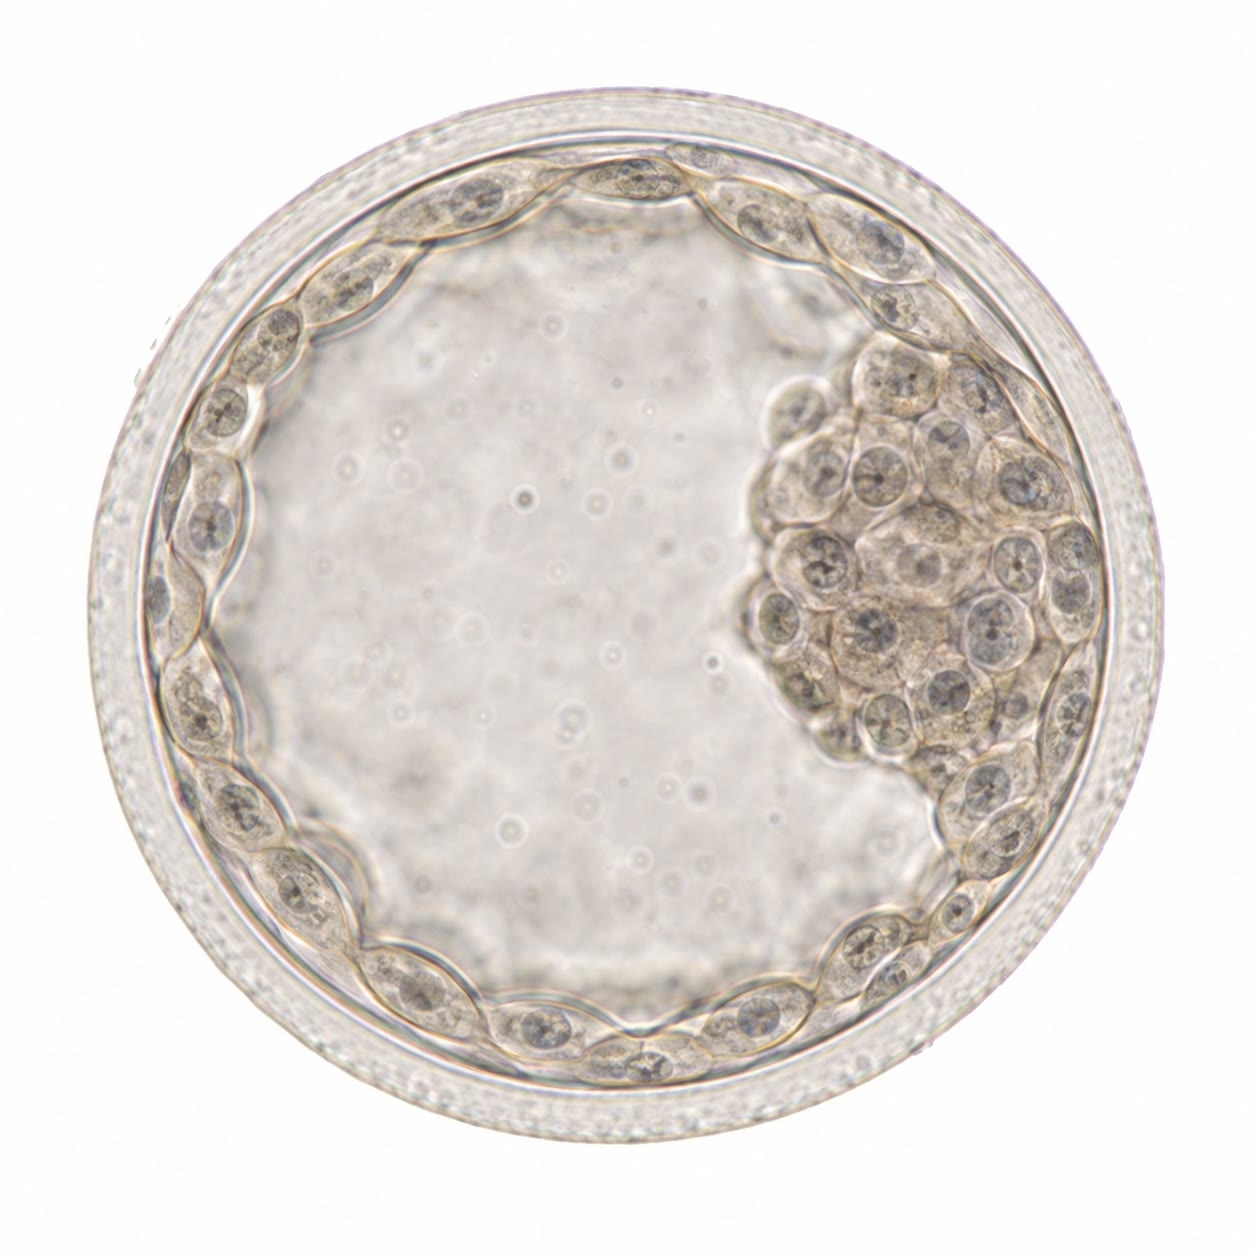
\includegraphics[width=0.42\linewidth]{images/book4/ai/b4-08-blastocyst.jpg}

{\small पाँचवें दिन एक \omterm{def:b2:mammal-reproduction:implantation}{कोरकपुटी}: गुहा के चारों ओर बाहरी \omterm{def:b2:mammal-reproduction:implantation}{पोषकोरक},
और एक ओर \omterm{def:b2:mammal-reproduction:implantation}{अंतःकोशिका पिंड} --- यानी भावी भ्रूण।}
\end{omfigure}

\begin{definition}[अपरा]\label{def:b2:mammal-reproduction:placenta}
\index{अपरा}\index{जरायु अंकुर}\index{नाभिरज्जु}
\emph{अपरा} ऐसा अंग है जो भ्रूण (जरायु, यानी
\omterm{def:b2:mammal-reproduction:implantation}{पोषकोरक} से) और माता (गर्भाशय का अस्तर) मिलकर बनाते हैं।
उँगली जैसे \emph{जरायु अंकुर}, जो शाखित होकर पूर्णावधि पर कोई
\qty{12}{m^2} की सतह बनाते हैं, मातृ रक्त की उन झीलों में लटकते हैं
जिन्हें गर्भाशयी धमनियाँ आधा लीटर प्रति मिनट पहुँचाती हैं; और हर अंकुर
के भीतर भ्रूणीय केशिकाएँ चलती हैं, जो \emph{नाभिरज्जु} की दो धमनियों और
एक शिरा से भ्रूण तक जुड़ी हैं। दोनों रक्त कभी नहीं मिलते:
उन्हें अंकुर की भित्ति अलग रखती है, यानी \omterm{def:b2:mammal-reproduction:implantation}{पोषकोरक} और केशिका अंतःस्तर के
कुछ माइक्रोमीटर, जिनके आरपार ऑक्सीजन,
$\mathrm{CO_2}$, जल, यूरिया और वसा-घुलनशील अणु विसरित होते हैं,
ग्लूकोज़ तथा ऐमीनो अम्ल वाहकों से ढोए जाते हैं, और मातृ
प्रतिरक्षियाँ (IgG) ग्राही से पहुँचाई जाती हैं, जो नवजात को उसके पहले
महीनों की प्रतिरक्षा देती हैं। अपरा एक ग्रंथि भी है: पहले
दिनों से \omterm{def:b2:mammal-reproduction:implantation}{पोषकोरक} \emph{मानव जरायु
गोनैडोट्रोपिन} (hCG) स्रावित करता है, जो \omterm{def:b2:mammal-reproduction:ovary}{पीत पिंड} को
प्रोजेस्टेरोन बनाते रखता है, और तीसरे महीने से अपरा स्वयं वह
प्रोजेस्टेरोन तथा एस्ट्रोजन बनाती है जो गर्भावस्था बनाए रखते हैं
(\cref{ch:b2:reproductive-hormones})। वह, वस्तुतः, नौ महीनों के लिए उगाया
और जन्म पर फेंक दिया गया एक फेफड़ा, एक आँत, एक वृक्क और एक अंतःस्रावी
ग्रंथि है।
\end{definition}

\begin{omfigure}
\begin{tikzpicture}[every node/.style={font=\scriptsize}, >=stealth]
  % maternal blood space
  \fill[omThm!12] (0,0) rectangle (8,3.6);
  \node[omThm!80!black, align=center] at (1.1,2.6) {मातृ रक्त\\(अंतराअंकुरी\\अवकाश)};
  % uterine wall at bottom
  \fill[omExo!30] (0,-0.6) rectangle (8,0); \node at (4,-0.3) {गर्भाशय की भित्ति (मातृ)};
  \draw[->, thick, omThm] (1.0,-0.6) -- (1.0,0.6); \node[omThm, anchor=west] at (1.05,0.3) {कुंडलित धमनी};
  \draw[->, thick, omDef!60!black] (7.0,0.6) -- (7.0,-0.6); \node[omDef!60!black, anchor=east] at (6.95,0.3) {गर्भाशयी शिरा};
  % chorionic plate at top
  \fill[omDef!20] (0,3.6) rectangle (8,4.4); \node at (4,4.0) {जरायु पट्टिका (भ्रूणीय)};
  % villi hanging down
  \foreach \x in {2.6,4.2,5.8} {
    \draw[thick, fill=omDef!8] (\x-0.35,3.6) -- (\x-0.4,1.4) .. controls (\x-0.4,0.9) and (\x+0.4,0.9) .. (\x+0.4,1.4) -- (\x+0.35,3.6);
    \draw[thick, omThm!70!black] (\x-0.15,3.6) -- (\x-0.15,1.5) .. controls (\x-0.15,1.25) and (\x+0.15,1.25) .. (\x+0.15,1.5) -- (\x+0.15,3.6);
    \foreach \y in {2.0,2.7} { \draw[thick, fill=omDef!8] (\x-0.4,\y) .. controls (\x-0.9,\y+0.1) and (\x-0.9,\y-0.4) .. (\x-0.4,\y-0.3); }
  }
  % umbilical vessels
  \draw[very thick, omThm!70!black] (4.2,4.4) -- (4.2,5.0) node[above, align=center] {नाभि शिरा (भ्रूण तक)\\और धमनियाँ};
  \draw[very thick, omDef!60!black] (3.9,4.4) -- (3.9,5.0); \draw[very thick, omDef!60!black] (4.5,4.4) -- (4.5,5.0);
  % exchange arrows
  \draw[<->, thick] (3.0,2.2) -- (3.75,2.2); \node[anchor=west, align=left] at (8.3,1.5) {भित्ति के आरपार: \textcolor{omThm}{O$_2$, ग्लूकोज़,}\\\textcolor{omThm}{ऐमीनो अम्ल, IgG} भ्रूण को;\\\textcolor{omDef!60!black}{CO$_2$, यूरिया} माता को};
  \node[anchor=west, align=left] at (8.3,3.0) {अंकुर की भित्ति: पोषकोरक\\+ भ्रूणीय केशिका अंतःस्तर,\\कुछ माइक्रोमीटर};
  \draw (6.2,2.5) -- (8.3,3.0);
\end{tikzpicture}

{\small \omterm{def:b2:mammal-reproduction:placenta}{अपरा}: भ्रूणीय केशिकाएँ ढोते भ्रूणीय अंकुर ऐसे
अवकाश में लटकते हैं जो कुंडलित धमनियों के मातृ रक्त से भरा है। दोनों
रक्त अंकुर की भित्ति के आरपार विनिमय करते हैं और कभी नहीं मिलते।}
\end{omfigure}

\begin{theorem}[अपरा के आरपार विनिमय]\label{thm:b2:mammal-reproduction:fick}
\index{फ़िक का नियम!अपरा}
$A$ क्षेत्रफल और $d$ मोटाई की किसी झिल्ली को पार करती कोई गैस
$J = K\,A\,\Delta P/d$ दर से चलती है, जिसमें $\Delta P$ उसके आंशिक दाब
का अंतर है और $K$ उस ऊतक की पारगम्यता। ऊतक में ऑक्सीजन
के लिए $K \approx \qty{3e-8}{mL/(cm.min.mmHg)}$; और $A =
\qty{12}{m^2}$, $d = \qty{3.5}{\micro m}$ तथा $\Delta P =
\qty{20}{mmHg}$ के साथ (अंतराअंकुरी अवकाश में मातृ \qty{40}{mmHg}
बनाम नाभि धमनी में \qty{20}{mmHg}), \omterm{def:b2:mammal-reproduction:placenta}{अपरा} प्रति मिनट
लगभग \qty{200}{mL} ऑक्सीजन पार करा सकती है, यानी उन
\qty{25}{mL/min} का कोई आठ गुना जो पूर्णावधि भ्रूण खपाता है। इसलिए
ऑक्सीजन-हस्तांतरण को विसरण नहीं बल्कि रक्त-प्रवाह सीमित करता है; और वह
भ्रूण कम ऑक्सीजन दाब पर काम करता है तथा अधिक बंधुता वाले हीमोग्लोबिन और
अधिक लाल-कोशिका संख्या से इसकी भरपाई करता है।
\end{theorem}
\begin{proof}
फ़िक का नियम कहता है कि अभिवाह प्रवणता $\Delta P/d$ के और क्षेत्रफल के
समानुपाती है; और स्थिरांक $K$ उस गैस की ऊतक में विलेयता तथा विसरण
गुणांक समेट लेता है। संख्याओं में:
$3\times 10^{-8}\times 1.2\times 10^{5}\times 20/(3.5\times 10^{-4})
= \qty{206}{mL/min}$, जिसमें $A$ \unit{cm^2} में और $d$ \unit{cm} में है।
भ्रूण की माँग \qty{3.5}{kg} के लिए लगभग \qty{7}{mL} प्रति किलोग्राम
प्रति मिनट है।
\end{proof}

\section{गर्भावधि, जन्म और स्तनपायन}

\begin{proposition}[गर्भावधि और जन्म]\label{prop:b2:mammal-reproduction:birth}
\index{गर्भावधि}\index{प्रसव}\index{ऑक्सीटोसिन}
गर्भावधि चूहे में \num{20} दिन, मनुष्य में \num{280} और हाथी में \num{660}
दिन चलती है --- मोटे तौर पर शरीर-द्रव्यमान की चौथाई घात की तरह, और
प्राइमेट अपने आकार के हिसाब से धीमे। उसे प्रोजेस्टेरोन बनाए रखता है,
जो गर्भाशयी पेशी को शांत और ग्रीवा को बंद रखता है। जन्म
(\emph{प्रसव}) का चालक भ्रूण स्वयं है: पूर्णावधि पर चढ़ता उसका
अधिवृक्क कॉर्टिसोल \omterm{def:b2:mammal-reproduction:placenta}{अपरा} को प्रोजेस्टेरोन से एस्ट्रोजन पर
हटा देता है, जो गर्भाशय को ऑक्सीटोसिन ग्राही और अंतराल संधियाँ दे देता है
और प्रोस्टाग्लैंडिन का मोचन आरंभ करा देता है। फिर एक \emph{धन
प्रतिपुष्टि} कमान सँभाल लेती है: शिशु का सिर ग्रीवा पर दबाव डालता है,
संवेदी तंत्रिकाएँ अधश्चेतक को संकेत देती हैं, पश्च पीयूष से
\emph{ऑक्सीटोसिन} छूटता है, गर्भाशय संकुचित होता है, सिर और ज़ोर से
दबाता है; और वह चक्र तब तक चढ़ता जाता है जब तक प्रसव न हो जाए, जिसके बाद
वह उद्दीपन समाप्त होता है और चक्र रुक जाता है --- शरीरक्रिया की उन थोड़ी
धन प्रतिपुष्टियों में से एक, और ऐसी जिसे किसी घटना पर समाप्त होना ही
पड़ता है। \omterm{def:b2:mammal-reproduction:placenta}{अपरा} कुछ मिनट बाद बाहर आती है।
\end{proposition}
\begin{proof}[प्रमाण-सामग्री]
फ़र्ग्युसन (1941) ने खरगोश में दिखाया कि ग्रीवा को फैलाने पर
गर्भाशयी संकुचन उठते हैं और मेरुरज्जु काट देने या पश्च पीयूष
हटा देने पर वह अनुक्रिया मिट जाती है: यानी ग्रीवा से पीयूष से गर्भाशय तक
एक तंत्रिका-अंतःस्रावी प्रतिवर्त। ऑक्सीटोसिन, जिसे
दू विन्यो ने 1953 में अलग किया और संश्लेषित किया, अब प्रसव प्रेरित करने
की मानक औषधि है।
\end{proof}

\begin{proposition}[स्तनपायन]\label{prop:b2:mammal-reproduction:lactation}
\index{स्तनपायन}\index{प्रोलैक्टिन}\index{दूध}
स्तन ग्रंथि, जो एक रूपांतरित स्वेद ग्रंथि है, गर्भावस्था में एस्ट्रोजन,
प्रोजेस्टेरोन और प्रोलैक्टिन से गढ़ी जाती है पर प्रोजेस्टेरोन उसे
स्रावित करने से रोके रखता है; और \omterm{def:b2:mammal-reproduction:placenta}{अपरा} के निकल जाने पर प्रोजेस्टेरोन
गिरता है तथा अग्र पीयूष के \emph{प्रोलैक्टिन} के नीचे वे
कूपिकाएँ दूध बनाने लगती हैं। दो प्रतिवर्त इस प्रक्रिया को चलाते हैं:
चूसना प्रोलैक्टिन का मोचन उकसाता है (जो संश्लेषण बनाए रखता है और
\omterm{def:b2:mammal-reproduction:ovary}{अंडोत्सर्ग} दबाता है) और ऑक्सीटोसिन का मोचन (जो कूपिकाओं के चारों ओर की
कोशिकाएँ सिकोड़कर दूध बाहर धकेलता है)। मानव दूध में
लगभग \qty{7}{\%} लैक्टोस, \qty{4}{\%} वसा, \qty{1}{\%} प्रोटीन और
\qty{2.9}{kJ/mL} होते हैं; और पहले दिनों का \emph{खीस}
प्रतिरक्षियों (IgA) से समृद्ध है, जो शिशु की आँत पर परत चढ़ा देती हैं।
कोई माता प्रतिदिन लगभग \qty{750}{mL} बनाती है, जिसका दाम कोई
\qty{2.5}{MJ} है --- यानी उसके भोजन का चौथाई भाग --- और वह भी
महीनों तक; स्तनपायन स्तनधारी जनन का सबसे महँगा भाग है और वही जिस पर इस
वर्ग का नाम है।
\end{proposition}

\section{दोनों लिंग बनाना}

\begin{proposition}[लिंग-निर्धारण और लिंग-विभेदन]\label{prop:b2:mammal-reproduction:sex}
\index{SRY}\index{प्रति-म्यूलरी हॉर्मोन}\index{लिंग विभेदन}
छठे सप्ताह तक किसी भी लिंग के मानव भ्रूण के पास वही साज-सामान होता है:
एक अविभेदित जनद, नलिकाओं के दो युग्म (\emph{वोल्फ़ीय}
और \emph{म्यूलरी}) और उदासीन बाह्य जननांग। Y गुणसूत्र का जीन
\emph{SRY} उस जनद में चालू होता है और उसे
\omterm{def:b2:mammal-reproduction:testis}{वृषण} बना देता है; उसके बिना वह जनद अंडाशय बन जाता है। फिर वह भ्रूणीय
\omterm{def:b2:mammal-reproduction:testis}{वृषण} दो काम करता है: उसकी \omterm{def:b2:mammal-reproduction:testis}{सर्टोली कोशिकाएँ}
\emph{\omterm{prop:b2:mammal-reproduction:sex}{प्रति-म्यूलरी हॉर्मोन}} स्रावित करती हैं, जो म्यूलरी नलिकाओं का
क्षय करा देता है, और उसकी \omterm{def:b2:mammal-reproduction:testis}{लाइडिग कोशिकाएँ} \emph{टेस्टोस्टेरोन} स्रावित
करती हैं, जो वोल्फ़ीय नलिकाएँ (यानी भावी अधिवृषण, शुक्रवाहिका,
शुक्राशय) बनाए रखता है और, डाइहाइड्रोटेस्टोस्टेरोन में बदलकर, बाह्य
जननांगों को शिश्न तथा वृषणकोष में ढाल देता है। दोनों संकेतों की
अनुपस्थिति में वोल्फ़ीय नलिकाएँ क्षीण हो जाती हैं, म्यूलरी नलिकाएँ
अंडवाहिनियाँ, गर्भाशय और ऊपरी योनि बन जाती हैं, और जननांग
मादा के रूप में विकसित होते हैं। मादा राह वही है जो तब ली जाती है जब कुछ
कहा ही न जाए: नर राह \omterm{def:b2:mammal-reproduction:testis}{वृषण} को सक्रिय रूप से थोपनी पड़ती है, और हर वह चरण
जिस पर यह थोपना विफल हो --- कोई उत्परिवर्ती SRY, कोई अनुपस्थित
हॉर्मोन-ग्राही --- ऐसा XY व्यक्ति देता है जिसकी काया मादा या मध्यवर्ती
होती है।
\end{proposition}
\begin{proof}[प्रमाण-सामग्री]
जोस्त (1947) ने खरगोश के भ्रूणों से गर्भाशय में ही, उनकी नलिकाओं के
विभेदित होने से पहले, जनद हटा दिए: किसी भी गुणसूत्रीय लिंग के बधिया
भ्रूणों में गर्भाशय, अंडवाहिनियाँ और मादा जननांग विकसित हुए।
किसी बधिया भ्रूण में रोपा गया टेस्टोस्टेरोन का एक रवा उस ओर की
वोल्फ़ीय नलिकाएँ बनाए रख सका पर म्यूलरी नलिकाएँ नहीं हटा सका; जबकि
ग्राफ़्ट किया गया कोई भ्रूणीय \omterm{def:b2:mammal-reproduction:testis}{वृषण} अपनी ओर दोनों कर सका:
यानी \omterm{def:b2:mammal-reproduction:testis}{वृषण} को मादा नलिकाएँ दबाने के लिए एक दूसरा, तब अज्ञात, कारक बनाना
ही चाहिए, जिसकी पहचान तीस वर्ष बाद \omterm{prop:b2:mammal-reproduction:sex}{प्रति-म्यूलरी
हॉर्मोन} के रूप में हुई। बाद में Y गुणसूत्र के एक छोटे टुकड़े के
लिंग-उलट प्रभाव ने उस स्विच को \emph{SRY} पर टिका दिया (1990), और
केवल \emph{Sry} जीन के साथ बनाया गया कोई XX चूहा नर के रूप में विकसित हुआ।
\end{proof}

\begin{omfigure}
\begin{tikzpicture}[every node/.style={font=\scriptsize}, >=stealth]
  \node[draw, rounded corners, fill=omExo!25, align=center] (g) at (0,0) {अविभेदित जनद\\दो नलिका-तंत्र};
  \node[draw, rounded corners, fill=omDef!15, align=center] (t) at (4.2,1.4) {वृषण\\(\emph{SRY} उपस्थित)};
  \node[draw, rounded corners, fill=omThm!15, align=center] (o) at (4.2,-1.4) {अंडाशय\\(\emph{SRY} नहीं)};
  \node[draw, rounded corners, fill=omDef!15, align=center] (amh) at (8.6,2.3) {AMH: म्यूलरी नलिकाएँ क्षीण};
  \node[draw, rounded corners, fill=omDef!15, align=center] (tst) at (8.6,0.6) {टेस्टोस्टेरोन: वोल्फ़ीय नलिकाएँ बची;\\DHT: नर बाह्य जननांग};
  \node[draw, rounded corners, fill=omThm!15, align=center] (f) at (8.6,-1.4) {कोई संकेत नहीं: वोल्फ़ीय नलिकाएँ क्षीण,\\म्यूलरी नलिकाएँ $\to$ अंडवाहिनियाँ, गर्भाशय;\\मादा जननांग};
  \draw[->, thick] (g) -- (t); \draw[->, thick] (g) -- (o);
  \draw[->, thick] (t) -- (amh); \draw[->, thick] (t) -- (tst); \draw[->, thick] (o) -- (f);
\end{tikzpicture}

{\small लैंगिक विभेदन: \emph{SRY} का बनाया \omterm{def:b2:mammal-reproduction:testis}{वृषण}
दो हॉर्मोनों से नर राह थोप देता है; और उनकी अनुपस्थिति में वह काया
मादा के रूप में विकसित होती है।}
\end{omfigure}

\section{अभ्यास}

\begin{exercise}[$\star$]\label{exo:b2:mammal-reproduction:1}
\omterm{def:b2:mammal-reproduction:testis}{शुक्राणुजनन} और \omterm{def:b2:mammal-reproduction:ovary}{अंडाणुजनन} की तुलना कीजिए: स्तंभ कोशिकाएँ कब विभाजित
होती हैं, एक \omterm{def:b2:meiosis-heredity:meiosis}{अर्धसूत्री विभाजन} कितने युग्मक देता है, कोई युग्मक बनने में
कितना समय लेता है, ठहराव कहाँ हैं, और जीवन भर में कितने युग्मक बनते
हैं।
\end{exercise}

\begin{exercise}[$\star$]\label{exo:b2:mammal-reproduction:2}
शुक्राणु के पटल पर पहुँचने से लेकर पहले समसूत्री विभाजन तक निषेचन के
चरण बताइए, और कहिए कि कौन-सा चरण बहुशुक्राणुता रोकता है।
\end{exercise}

\begin{exercise}[$\star$]\label{exo:b2:mammal-reproduction:3}
\omterm{def:b2:mammal-reproduction:implantation}{कोरकपुटी} की दोनों कोशिका-आबादियाँ और हर एक की नियति
बताइए। \omterm{def:b2:mammal-reproduction:implantation}{रोपण} किस दिन आरंभ होता है, और किस हॉर्मोन ने गर्भाशय
तैयार किया होगा?
\end{exercise}

\begin{exercise}[$\star$]\label{exo:b2:mammal-reproduction:4}
इनमें से हर एक के लिए बताइए कि वह \omterm{def:b2:mammal-reproduction:placenta}{अपरा} पार करता है या नहीं और
कैसे: ऑक्सीजन, ग्लूकोज़, मातृ लाल कोशिकाएँ, IgG प्रतिरक्षी, यूरिया,
ऐल्कोहॉल, अधिकांश जीवाणु।
\end{exercise}

\begin{exercise}[$\star\star$]\label{exo:b2:mammal-reproduction:5}
प्रति शुक्राणु $\pi = 10^{-8}$ के साथ, $3\times 10^{8}$, $10^{8}$,
$4\times 10^{7}$ और $10^{7}$ शुक्राणु-संख्याओं के लिए निषेचन की
प्रायिकता निकालिए। वह किस संख्या पर एक-आधे से
नीचे गिरती है? यह शुक्राणु-संख्या के सापेक्ष उर्वरता की मात्रा--अनुक्रिया
के आकार के बारे में क्या कहता है?
\end{exercise}

\begin{exercise}[$\star\star$]\label{exo:b2:mammal-reproduction:6}
कोई बालिका $10^{6}$ अंडाणुकों के साथ जन्म लेती है, यौवनारंभ (आयु 13) पर
उसके पास \num{300000} होते हैं और 50 पर लगभग \num{1000}, और वह \num{400}
अंडोत्सर्जित कर चुकी होती है। यौवनारंभ से पहले और बाद पुटकनाश की माध्य दर
(प्रतिदिन खोए अंडाणुक) निकालिए, और \omterm{def:b2:mammal-reproduction:ovary}{अंडोत्सर्ग} की दर से तुलना कीजिए।
\end{exercise}

\begin{exercise}[$\star\star$]\label{exo:b2:mammal-reproduction:7}
भ्रूणीय हीमोग्लोबिन का अर्ध-संतृप्ति दाब $P_{50} =
\qty{19}{mmHg}$ है और वयस्क हीमोग्लोबिन का \qty{27}{mmHg}; और संतृप्ति
$S = P^{n}/(P_{50}^{n} + P^{n})$ लीजिए, जिसमें $n = 2.7$ है।
नाभि शिरा के दाब \qty{30}{mmHg} पर दोनों संतृप्तियाँ
निकालिए, और उस लाभ को समझाइए।
\end{exercise}

\begin{exercise}[$\star\star$]\label{exo:b2:mammal-reproduction:8}
hCG मातृ रक्त में \omterm{def:b2:mammal-reproduction:implantation}{रोपण} पर (निषेचन के बाद दिन 7)
लगभग \qty{1}{IU/L} पर प्रकट होती है और हर दो दिन में दुगुनी होती है; और
कोई गर्भावस्था-परीक्षण \qty{25}{IU/L} पकड़ता है। निषेचन के बाद किस दिन
वह परीक्षण धनात्मक होता है? और अंतिम रजःस्राव के बाद
(\omterm{def:b2:mammal-reproduction:ovary}{अंडोत्सर्ग} दिन 14 पर) किस दिन?
\end{exercise}

\begin{exercise}[$\star\star$]\label{exo:b2:mammal-reproduction:9}
प्रमेय का अपरा-ऑक्सीजन हस्तांतरण ऐसी किसी
\omterm{def:b2:mammal-reproduction:placenta}{अपरा} के लिए फिर से निकालिए जो \qty{6}{m^2} की हो और जिसके अंकुर की
भित्ति \qty{10}{\micro m} की हो, जैसा कुछ विकृतियों में होता है, और भ्रूण
की माँग से तुलना कीजिए। उस भ्रूण का क्या होता है?
\end{exercise}

\begin{exercise}[$\star\star\star$]\label{exo:b2:mammal-reproduction:10}
इनके नलिका-तंत्र और बाह्य जननांगों की भविष्यवाणी कीजिए: (क) ऐसा XY
भ्रूण जिसकी कोशिकाओं में टेस्टोस्टेरोन-ग्राही नहीं है; (ख) ऐसा XY भ्रूण
जिसमें \omterm{prop:b2:mammal-reproduction:sex}{प्रति-म्यूलरी हॉर्मोन} नहीं है; (ग) ऐसा XX भ्रूण जो अपने
अधिवृक्कों के ऊँचे टेस्टोस्टेरोन के सामने रहा है; (घ) ऐसा XX भ्रूण जो
किसी X गुणसूत्र पर \emph{SRY} ढोता है। हर एक को जोस्त के परिणामों से समझाइए।
\end{exercise}

\begin{exercise}[$\star\star\star$]\label{exo:b2:mammal-reproduction:11}
समरूप जुड़वाँ तब उठते हैं जब कोई एक भ्रूण बँट जाए। वह दिन 3 से पहले
बँटे तो जुड़वाँ की \omterm{def:b2:mammal-reproduction:placenta}{अपरा} और थैलियाँ अलग होती हैं; दिन 4 और
8 के बीच, एक \omterm{def:b2:mammal-reproduction:placenta}{अपरा} और दो थैलियाँ; दिन 8 और 13 के बीच, एक \omterm{def:b2:mammal-reproduction:placenta}{अपरा} और
एक थैली; और उसके बाद वे जुड़े हुए होते हैं। समरूप जुड़वाँ की किसी शृंखला
में \qty{30}{\%} की \omterm{def:b2:mammal-reproduction:placenta}{अपरा} अलग होती है, \qty{68}{\%} की एक \omterm{def:b2:mammal-reproduction:placenta}{अपरा} और
दो थैलियाँ, और \qty{2}{\%} की एक थैली। निकालिए कि विकास की कौन-सी अवस्था
सबसे अधिक बार बँटती है, और \omterm{def:b2:mammal-reproduction:implantation}{कोरकपुटी} के पदों में समझाइए कि हर
स्थिति में कौन-सी संरचनाएँ साझा होती हैं।
\end{exercise}

\begin{exercise}[$\star\star\star$]\label{exo:b2:mammal-reproduction:12}
मार्सूपियल कुछ ही सप्ताह बाद सेम के दाने जितने बच्चे को जन्म देते हैं जो
अपनी वृद्धि थैली में किसी चुचुक पर पूरी करता है; जबकि अपरायुक्त स्तनधारी
लंबी गर्भावधि रखते हैं और बड़े बच्चे को जन्म देते हैं। दोनों
रणनीतियों की तुलना मातृ लागत, जोखिम, और किसी बुरी ऋतु में माता के
लिटर छोड़ देने की क्षमता के पदों में कीजिए, और सुझाइए कि ऑस्ट्रेलिया को
छोड़कर हर महाद्वीप पर अपरायुक्तों ने मार्सूपियलों को क्यों हटा दिया।
\end{exercise}

\section{समस्या: संख्याओं में एक गर्भावस्था}

\begin{problem}[{सप्तांत समस्या --- किसी मानव गर्भावस्था का शुक्राणु से
दूध तक पीछा, निषेचन की प्रायिकताओं, रोपण के समय और उसके हॉर्मोन,
अपरा की विनिमय-क्षमता, तथा गर्भावधि और स्तनपायन की ऊर्जा-लागत से होकर,
और अंत निषेचन की प्रायिकता, परीक्षण के धनात्मक होने के दिन, अपरा की
ऑक्सीजन-गुंजाइश और एक दिन के दूध की लागत पर}]
\label{pb:b2:mammal-reproduction:1}
आँकड़े: प्रति स्खलन $3\times 10^{8}$ शुक्राणु, और हर एक के अंडाणु तक
पहुँचने की प्रायिकता $10^{-8}$; शुक्राणु \qty{50}{\micro m/s} से तैरते
हैं; तुंबिका ग्रीवा से \qty{15}{cm} दूर है। \omterm{def:b2:mammal-reproduction:implantation}{रोपण} (दिन 7) पर hCG
\qty{1}{IU/L}, हर \qty{2}{d} में दुगुनी, और परीक्षण-देहली
\qty{25}{IU/L}। पूर्णावधि पर \omterm{def:b2:mammal-reproduction:placenta}{अपरा}: \qty{12}{m^2}, भित्ति
\qty{3.5}{\micro m}, $K_{\mathrm{O_2}} = \qty{3e-8}{mL/(cm.min.mmHg)}$,
$\Delta P = \qty{20}{mmHg}$; भ्रूण \qty{3.5}{kg}, जो प्रति किलोग्राम
प्रति मिनट \qty{7}{mL} ऑक्सीजन खपाता है; \omterm{def:b2:mammal-reproduction:placenta}{अपरा} तक मातृ
रक्त-प्रवाह \qty{500}{mL/min}, जो प्रति मिलिलिटर रक्त \qty{0.16}{mL}
ऑक्सीजन ढोता है। ग्लूकोज़: भ्रूण प्रति किलोग्राम प्रति मिनट \qty{5}{mg}
लेता है; मातृ रक्त \qty{0.9}{g/L}। दूध: \qty{750}{mL/d}
\qty{2.9}{kJ/mL} पर, \qty{80}{\%} दक्षता से बना; शिशु प्रतिदिन
\qty{30}{g} ऊतक \qty{6}{kJ/g} जमा करके बढ़ता है और \qty{4}{kg} पर
अनुरक्षण पर \qty{300}{kJ/kg/d} ख़र्च करता है।

\medskip
\noindent\textbf{भाग I --- निषेचन।}
\begin{enumerate}
  \item अंडाणु तक पहुँचते शुक्राणुओं की माध्य संख्या और निषेचन की
        प्रायिकता निकालिए।
  \item दो या अधिक के पहुँचने की प्रायिकता निकालिए, और बताइए कि
        \omterm{prop:b2:mammal-reproduction:fertilisation}{वल्कुटीय अभिक्रिया} के बिना क्या होता।
  \item किसी शुक्राणु को तुंबिका तक तैरने में कितना समय लगता? शुक्राणु
        वहाँ \qty{30}{min} के भीतर मिल जाते हैं: उन्हें कौन ले जाता है?
  \item तुंबिका तक कुछ सौ शुक्राणु ही पहुँचते हैं। वह स्खलन का कितना
        अंश है, और बाक़ी कहाँ खो जाते हैं?
  \item कोई अंडाणु लगभग एक दिन निषेच्य रहता है, और शुक्राणु उस मार्ग
        में लगभग तीन दिन जीते हैं। चक्र के कितने दिनों में संभोग से
        गर्भाधान हो सकता है?
  \item किसी पुरुष की संख्या गिरकर $5\times 10^{7}$ हो जाती है। प्रति
        चक्र निषेचन की प्रायिकता, और गर्भाधान तक चक्रों की प्रत्याशित
        संख्या (ज्यामितीय नियम), फिर से निकालिए।
  \item समझाइए कि भ्रूण की सूत्रकणिकाएँ अंडाणु देता है, शुक्राणु क्यों
        नहीं।
\end{enumerate}

\medskip
\noindent\textbf{भाग II --- \omterm{def:b2:mammal-reproduction:implantation}{रोपण} और उसका हॉर्मोन।}
\begin{enumerate}[resume]
  \item यदि हर विदलन विभाजन में \qty{16}{h} लगें, तो दिन 5 तक कितने
        विभाजन हो चुके हैं? कितनी कोशिकाएँ?
  \item निषेचन के बाद किस दिन hCG परीक्षण-देहली तक पहुँचती है? और
        अंतिम रजःस्राव के बाद (\omterm{def:b2:mammal-reproduction:ovary}{अंडोत्सर्ग} दिन 14 पर)?
  \item hCG को \omterm{def:b2:mammal-reproduction:implantation}{रोपण} के कुछ ही दिनों में क्यों प्रकट होना ही चाहिए? और
        न हो तो \omterm{def:b2:mammal-reproduction:ovary}{पीत पिंड} का, और गर्भावस्था का, क्या
        होता है?
  \item hCG सप्ताह 10 के आसपास \qty{1e5}{IU/L} के पास शिखर छूती है और
        फिर गिरती है। वह \omterm{def:b2:mammal-reproduction:implantation}{रोपण} से कितने दुगुनेपन हैं, और वह
        उसके बाद गर्भावस्था खोए बिना क्यों गिर सकती है?
  \item आधे गर्भाधान \omterm{def:b2:mammal-reproduction:implantation}{रोपण} पर या उससे पहले खो जाते हैं,
        अधिकतर असुगुणित अंडाणुओं से। \omterm{def:b2:mammal-reproduction:ovary}{अंडाणुजनन} की समय-रेखा
        से समझाइए कि असुगुणिता शुक्राणुओं की अपेक्षा अंडाणुओं में अधिक
        आम क्यों है।
  \item जुड़वाँ: कोई भ्रूण जो दिन 6 पर बँटता है। बताइए कि वे जुड़वाँ
        \omterm{def:b2:mammal-reproduction:placenta}{अपरा} और उल्ब थैली साझा करते हैं या नहीं।
\end{enumerate}

\medskip
\noindent\textbf{भाग III --- \omterm{def:b2:mammal-reproduction:placenta}{अपरा}।}
\begin{enumerate}[resume]
  \item अधिकतम विसरण ऑक्सीजन-हस्तांतरण निकालिए।
  \item भ्रूण की ऑक्सीजन-माँग और विसरण की गुंजाइश निकालिए।
  \item \omterm{def:b2:mammal-reproduction:placenta}{अपरा} तक मातृ रक्त-प्रवाह प्रति मिनट कितनी ऑक्सीजन
        पहुँचाता है, निकालिए। उस माँग को पूरा करने के लिए उसका कितना अंश
        निकालना पड़ता है?
  \item भ्रूण की ग्लूकोज़-माँग ग्राम प्रतिदिन में, और उतना ग्लूकोज़
        रखने वाले मातृ रक्त का आयतन, निकालिए। दैनिक मातृ अपरा-प्रवाह से
        तुलना कीजिए।
  \item भ्रूण का रक्त \omterm{def:b2:mammal-reproduction:placenta}{अपरा} से \qty{30}{mmHg} ऑक्सीजन पर
        निकलता है। वह उस दाब पर, जो किसी वयस्क को बेहोश कर देता, दम क्यों
        नहीं तोड़ता?
  \item ऐसी दो बातें बताइए जो \omterm{def:b2:mammal-reproduction:placenta}{अपरा} करती है और उस समय भ्रूण का
        कोई दूसरा अंग नहीं कर सकता, और एक जो वह नहीं कर सकती।
\end{enumerate}

\medskip
\noindent\textbf{भाग IV --- जन्म और दूध।}
\begin{enumerate}[resume]
  \item प्रसव की धन प्रतिपुष्टि का वर्णन कीजिए और समझाइए कि वह
        पूर्णावधि से पहले क्यों नहीं भड़क उठती।
  \item एक दिन के दूध की ऊर्जा और उसे बनाने में माता की ख़र्च होती
        ऊर्जा निकालिए।
  \item शिशु का दैनिक ऊर्जा-बजट (वृद्धि जमा अनुरक्षण) निकालिए और
        मिलते दूध से तुलना कीजिए।
  \item नौ महीने के स्तनपायन की माता की कुल ऊर्जा-लागत निकालिए, और
        गर्भावस्था की अपनी \qty{300}{MJ} लागत से तुलना कीजिए।
  \item समझाइए कि चूसना \omterm{def:b2:mammal-reproduction:ovary}{अंडोत्सर्ग} की वापसी क्यों टालता है, और
        गर्भनिरोध-रहित आबादियों में इसका क्या महत्व है।
  \item परिणाम बताइए: निषेचन की प्रायिकता, परीक्षण के धनात्मक होने का
        दिन, \omterm{def:b2:mammal-reproduction:placenta}{अपरा} की ऑक्सीजन-गुंजाइश, और एक दिन के दूध की
        लागत।
\end{enumerate}
\end{problem}
